% Fig 2.2 — Query Enhancement taxonomy
\documentclass[border=4pt]{standalone}
\usepackage{tikz}
% Shared TikZ style for thesis figures.
% Each fig_*.tex \input{} this file after \usepackage{tikz}.
% Defines a muted, examiner-friendly color palette and semantic box styles.

\usepackage{xcolor}
\usepackage{fontawesome5}
\usetikzlibrary{positioning, arrows.meta, shapes.geometric, calc, fit, backgrounds}

% ─── Palette ───────────────────────────────────────────────────────────
% Each role has a stroke color (dark) and a fill color (very light).
% Designed to be grayscale-safe — lightness differs enough that B&W printing
% still preserves the distinction.

\definecolor{thQueryS}{HTML}{4A6FA5}    \definecolor{thQueryF}{HTML}{E8EEF6}   % query / input
\definecolor{thLLMS}{HTML}{6D4A8F}      \definecolor{thLLMF}{HTML}{ECE5F2}     % LLM / generation
\definecolor{thRetS}{HTML}{3D7A4F}      \definecolor{thRetF}{HTML}{E4EFE7}     % retriever
\definecolor{thDataS}{HTML}{6A6A6A}     \definecolor{thDataF}{HTML}{F1F1F1}    % corpus / data
\definecolor{thFusionS}{HTML}{A05A30}   \definecolor{thFusionF}{HTML}{F4E8DF}  % fusion
\definecolor{thOutS}{HTML}{1F6F8A}      \definecolor{thOutF}{HTML}{DEEAEF}     % output / final
\definecolor{thHiS}{HTML}{0D4D63}       \definecolor{thHiF}{HTML}{C8D9DF}      % highlighted (our contribution)
\definecolor{thMuted}{HTML}{5C5C5C}

% ─── Box styles ────────────────────────────────────────────────────────
% Usage in tikzpicture options:  query/.style={thQuery}, llm/.style={thLLM}, ...
% Or directly on nodes:          \node[thLLM] (m) {...};
\tikzset{
  thBase/.style={rectangle, draw, rounded corners=2pt,
                 minimum width=28mm, minimum height=10mm,
                 align=center, font=\small, line width=0.6pt,
                 inner sep=4pt},
  thQuery/.style={thBase, draw=thQueryS, fill=thQueryF},
  thLLM/.style={thBase, draw=thLLMS, fill=thLLMF},
  thRet/.style={thBase, draw=thRetS, fill=thRetF},
  thData/.style={cylinder, shape border rotate=90, aspect=0.3, draw=thDataS, fill=thDataF,
                 minimum width=24mm, minimum height=12mm, align=center, font=\small, line width=0.6pt},
  thFusion/.style={thBase, draw=thFusionS, fill=thFusionF},
  thOut/.style={thBase, draw=thOutS, fill=thOutF},
  thHi/.style={thBase, draw=thHiS, fill=thHiF, line width=1pt},
  thArrow/.style={-{Stealth[length=2.5mm]}, line width=0.7pt, draw=thMuted},
  thLabel/.style={font=\footnotesize\itshape, color=thMuted},
  thStage/.style={font=\bfseries\footnotesize, color=thMuted},
}

% ─── Icon helpers ──────────────────────────────────────────────────────
% Tiny FontAwesome icons that can sit inside a node prefix.
% Usage:  \node[thQuery] {\thIconQuery~User query};
\newcommand{\thIconQuery}{\textcolor{thQueryS}{\faSearch}}
\newcommand{\thIconUser}{\textcolor{thQueryS}{\faUser}}
\newcommand{\thIconLLM}{\textcolor{thLLMS}{\faBrain}}
\newcommand{\thIconRet}{\textcolor{thRetS}{\faNetworkWired}}
\newcommand{\thIconCorpus}{\textcolor{thDataS}{\faDatabase}}
\newcommand{\thIconFusion}{\textcolor{thFusionS}{\faCodeBranch}}
\newcommand{\thIconOut}{\textcolor{thOutS}{\faFile}}
\newcommand{\thIconEval}{\textcolor{thOutS}{\faChartBar}}
\newcommand{\thIconStar}{\textcolor{thHiS}{\faStar}}
\newcommand{\thIconCog}{\textcolor{thMuted}{\faCog}}


\begin{document}
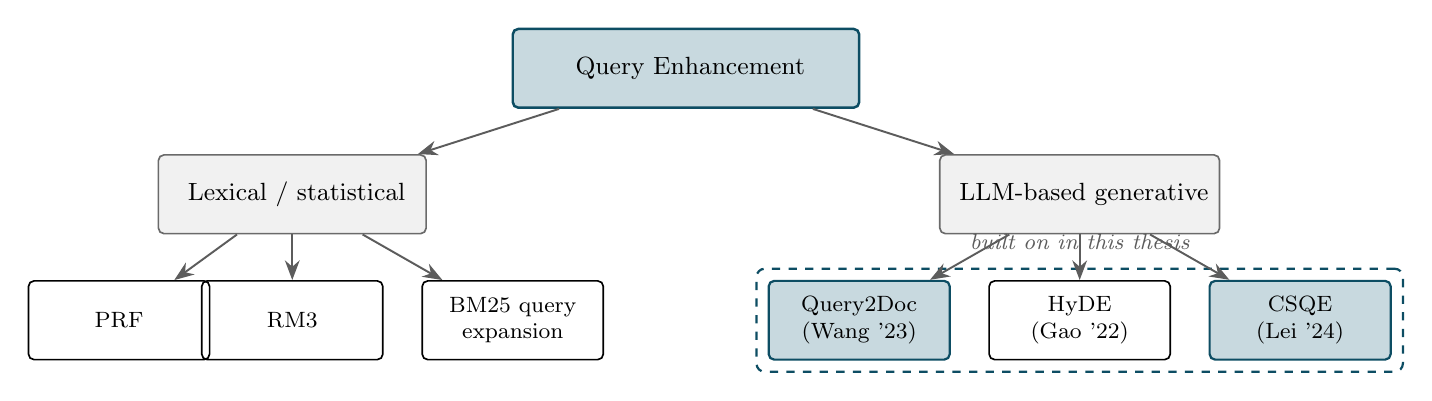
\begin{tikzpicture}[
    root/.style={thBase, draw=thHiS, fill=thHiF, minimum width=44mm, line width=0.9pt},
    branch/.style={thBase, fill=thDataF, draw=thDataS, minimum width=34mm},
    leaf/.style={thBase, minimum width=23mm, font=\footnotesize},
    thesis/.style={thBase, draw=thHiS, fill=thHiF, minimum width=23mm, font=\footnotesize, line width=0.8pt}
]
  \node[root] (root) at (0, 0) {\thIconStar~Query Enhancement};

  \node[branch] (lex) at (-50mm, -16mm) {\thIconCog~Lexical / statistical};
  \node[branch] (gen) at (50mm, -16mm) {\thIconLLM~LLM-based generative};

  \node[leaf] (prf) at (-72mm, -32mm) {PRF};
  \node[leaf] (rm3) at (-50mm, -32mm) {RM3};
  \node[leaf] (bm25exp) at (-22mm, -32mm) {BM25 query\\expansion};

  \node[thesis] (q2d) at (22mm, -32mm) {Query2Doc\\(Wang '23)};
  \node[leaf] (hyde) at (50mm, -32mm) {HyDE\\(Gao '22)};
  \node[thesis] (csqe) at (78mm, -32mm) {CSQE\\(Lei '24)};

  \draw[thArrow] (root) -- (lex);
  \draw[thArrow] (root) -- (gen);
  \draw[thArrow] (lex) -- (prf);
  \draw[thArrow] (lex) -- (rm3);
  \draw[thArrow] (lex) -- (bm25exp);
  \draw[thArrow] (gen) -- (q2d);
  \draw[thArrow] (gen) -- (hyde);
  \draw[thArrow] (gen) -- (csqe);

  \begin{scope}[on background layer]
    \node[draw=thHiS, dashed, rounded corners=3pt, fit=(q2d) (csqe), inner sep=4pt, line width=0.8pt] (thesisbox) {};
  \end{scope}
  \node[thLabel, above=1mm of thesisbox] {built on in this thesis};
\end{tikzpicture}
\end{document}
